\chapter{\xlabel{pipeline}The SCUBA-2 Pipeline}
\label{sec:pipe}

\section{\xlabel{pl_overview}Pipeline overview}

SCUBA-2 data reduction pipelines have been developed based on the
existing \oracdr\ pipeline (Cavanagh et al., 2008\cite{oracdr}) used
for ACSIS. There are three distinct pipelines currently utilised by
SCUBA-2. Users will likely only need to run the science pipeline. The
other two pipelines are designed to run at the JCMT---the quick-look (QL) and
summit pipelines. The latter two are run in real time at the JCMT
during data acquisition.

\begin{itemize}
\item The science pipeline has access to all the data observed for a
given project and adopts a best-possible reduction approach. Images are
made for each complete observation which are combined to create the final
image. Users wishing to reduce their own data should use this pipeline.
This pipeline is responsible for producing the reduced data that is
accessible to users via CADC.
\item The QL runs quality assurance checks on the data as it comes in.
For science data it calculates the noise between 2\,Hz and 10\,Hz,
along with the NEP and effective NEP, for each 30-second scan. These
values undergo quality-assurance checks to ensure SCUBA-2 is within
an acceptable operating range.
\item The summit pipeline is designed to provide a quick map of the
data, it does this by running fewer iterations and chunking the data
more. This is a useful guide to observers who wish to check the
quality of their data.

\end{itemize}

The manual for the SCUBA-2 pipeline can be found at \pipelinesun,
while the pipeline software comes as part of the \starlink\ suite.


\section{\xlabel{science_pl}The Science Pipeline}

The science pipeline will perform the following:
\vspace{-0.3cm}
\begin{itemize}\itemsep-0.3em
\item Run the iterative map-maker.
\item Apply the FCF to calibrate to mJy/beam.
\item Co-add multiple observations of the same object.
\item Apply the matched-filter (blank-field configuration file only)
\item Run a source-finding algorithm.
\end{itemize}

\subsection{\xlabel{pl_output}Pipeline recipes}
\label{sec:recipes}

When a project is initially created and MSBs (Minimum Scheduling Blocks)
are created in the Observing Tool, the PI can select a pipeline recipe to assign
to the data. When the data are run through the science pipeline this
recipe is then called by default. This can be overridden on the command
line---see \cref{Section}{sec:parameterfile}{Changing the defaults}.
Described below are the five main \oracdr\ science recipes.

\subsection{\xlabel{extsources}\drrecipe{REDUCE\_SCAN}}

\textbf{configuration file: \file{dimmconfig\_jsa\_generic.lis}}

This recipe uses the configuration file \jsageneric\ for \makemap, unless
the sources is identified as a calibrator. After all observations have
been processed the data are co-added and calibrated in mJy/beam using
the default FCF. The noise and NEFD properties for the co-add are
calculated and written to log files (\file{log.noise} and
\file{log.nefd} respectively). Finally, the \cupid\ task \findclumps\
is run using the FellWalker algorithm (Berry, 2015\cite{fellwalker}) to
create a source catalogue.

For calibrators, \file{dimmconfig\_bright\_compact.lis} is used and
FCFs are derived from the map.


\subsection{\xlabel{extsources}\drrecipe{REDUCE\_SCAN\_CHECKRMS}}

\textbf{Configuration file: \file{dimmconfig\_jsa\_generic.lis}}

This recipe is the same as \drrecipe{REDUCE\_SCAN}, but includes extra
performance estimations determined by \drrecipe{SCUBA2\_CHECK\_RMS}
(see \picard's \xref{\drrecipe{SCUBA2\_CHECK\_RMS}}{sun265}{SCUBA2_CHECK_RMS}). These extra
metrics are written to a log file \file{log.checkrms}. Running
\drrecipe{SCUBA2\_CHECK\_RMS} in the pipeline, rather than as a
standalone \picard\ recipe, allows it to calculate results for
co-added maps.


\subsection{\xlabel{extsources}\drrecipe{REDUCE\_SCAN\_EXTENDED\_SOURCES}}

\textbf{Configuration file: \file{dimmconfig\_bright\_extended.lis}}

This is the recipe for processing extended sources. Multiple
observations are co-added and the output map is calibrated in units of
mJy/arcsec$^2$. This recipe also performs a source-finder routine; the
results are written as a FITS catalogue (with file extension
\file{.FIT}) which can be read as a local catalogue into \gaia.

\subsection{\xlabel{faint}\drrecipe{REDUCE\_SCAN\_FAINT\_POINT\_SOURCES}}

\textbf{Configuration file: \file{dimmconfig\_blank\_field.lis}}

This is the recipe for processing maps containing faint compact
sources. This time the configuration file called by \makemap\ is
\file{dimmconfig\_blank\_field.lis} and the map calibrated in
mJy/beam.  The output map is further processed with a matched filter,
then the S/N is taken to enhance point sources.  A map is written out
at each step.  This recipe also performs a source finder routine; the
results are written as a FITS catalogue (with file extension
\file{.FIT}) which can be read as a local catalogue into \gaia.

\subsection{\xlabel{brightcom}\drrecipe{REDUCE\_SCAN\_ISOLATED\_SOURCE}}

\textbf{Configuration file: \file{dimmconfig\_bright\_compact.lis}}

This is the recipe used for processing calibrator data. It can also
be used for any map of a single bright, isolated source at the
tracking position. 

This reduction constrains the map to zero beyond a radius of 1 arc-min
from the source centre. See \cref{Section}{sec:brightcompact}{dimmconfig\_bright\_compact.lis}


\subsection{\xlabel{faintjk}\drrecipe{FAINT\_POINT\_SOURCES\_JACKKNIFE}}

\textbf{Configuration file: \file{dimmconfig\_blank\_field.lis}}

This recipe uses a
\htmladdnormallink{jack-knife}{http://en.wikipedia.org/wiki/Jackknife_resampling}
method to remove residual low-spatial frequency noise and create an
optimal matched-filtered output map. The map-maker is run twice, first
as a standard reduction using \file{dimmconfig\_blank\_field.lis} (and
calibrated in mJy/beam), and the second time with a fake source added
to the time series. This creates a signal map and an effective PSF
map. A jack-knife map is generated from two halves of the dataset and
the maps are `whitened' by the removal of the residual 1/\emph{f}
noise. The whitened signal map is processed with the matched filter
using the whitened PSF map as the PSF input. The data are calibrated
in mJy/beam using a corrected FCF.  See \cref{Section}{sec:jk}{Example
  2 -- Advanced pipeline method} for a more-detailed description of
this recipe and the files produced.


\section{\xlabel{running_pl}Running the Science Pipeline}
\label{sec:plsteps}


\begin{aligndesc}
\item[Step~1:]
\textbf{Initialise ORAC-DR}

For 850 micron data, this is done by:
\begin{terminalv}
% oracdr_scuba2_850 -cwd
\end{terminalv}

\vspace{0.2cm}

For 450 micron data, this is done by:

\begin{terminalv}
% oracdr_scuba2_450 -cwd
\end{terminalv}

\vspace{0.2cm}

\item[Step 2:]
\textbf{Set environment variables}

These ensure the data are read from and written to the right
places. Many are set automatically when the pipeline is initialised
but others must be set manually. Details of the optional variables are
given in \pipelinesun\ but the three main ones are:

\begin{itemize}\itemsep-0.1em
\item \envvar{STARLINK\_DIR} -- Location of your Starlink installation.
\item \envvar{ORAC\_DATA\_IN} -- The location where the data should be read from.
If you are supplying a text file listing the raw data this should be the
location of that file.
\item \envvar{ORAC\_DATA\_OUT} -- The location where the data products should be
written. Also used as the location for a user-specified configuration file.
\end{itemize}

\item[Step 3:]
\textbf{Run the pipeline}

This is done by:
\begin{terminalv}
% oracdr  -loop file -files <list_of_files>
\end{terminalv}

\vspace{0.2cm}

where the list of files that you wish to reduce can be
an individual or multiple observations.

\end{aligndesc}


\begin{tip}
  If you run with -verbose on the command line then you will obtain all messages
 from the Starlink engines (rather than just ORAC-DR messages). This is
 particularly useful for understanding what is occurring during the map-maker stage
 of reduction. This is particularly recommended for new users.
\end{tip}

When executing the \oracdr command a new Xwindow will appear within which
will contain the pipeline output, as shown in Figures
\ref{pipeline-oracdr-1}--\ref{pipeline-oracdr-4}.

\begin{figure}
\begin{center}
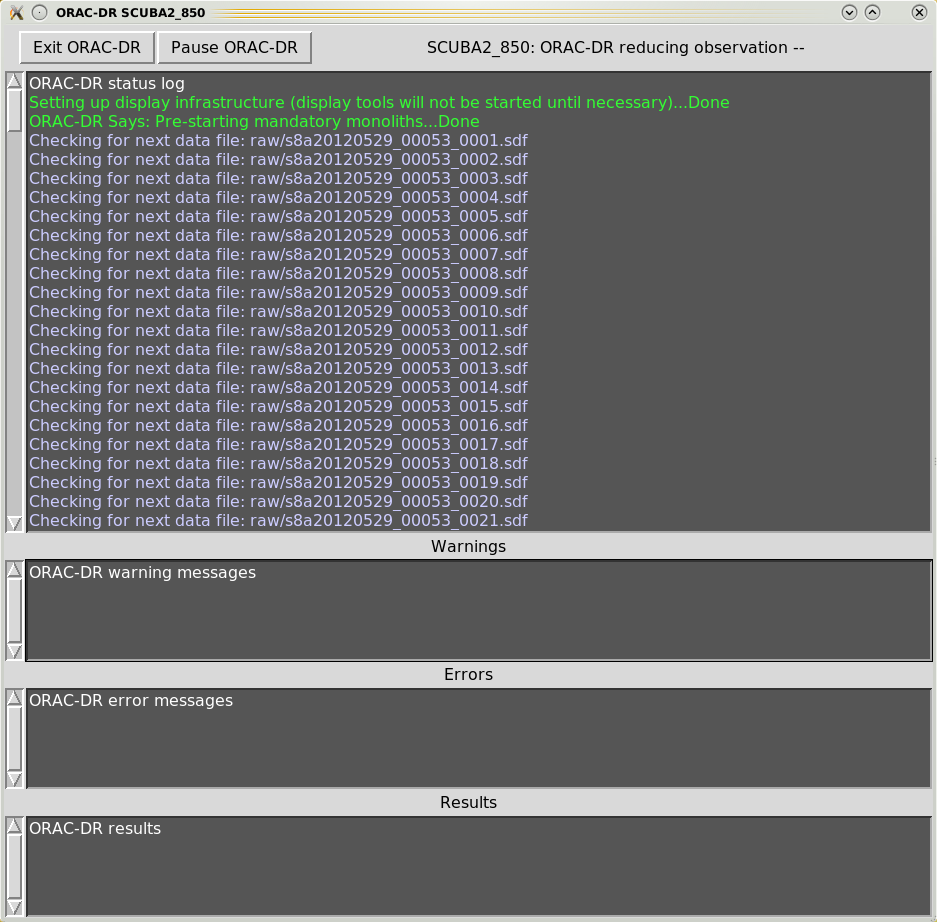
\includegraphics[width=0.7\linewidth]{sc21-pipeline-oracdr-1}
\caption[Output from the pipeline]{The Xwindows output from the \oracdr\
pipeline showing the initial log---here we see the pipeline is checking
for the raw files. \label{pipeline-oracdr-1}}
\end{center}
\end{figure}

\begin{figure}
\begin{center}
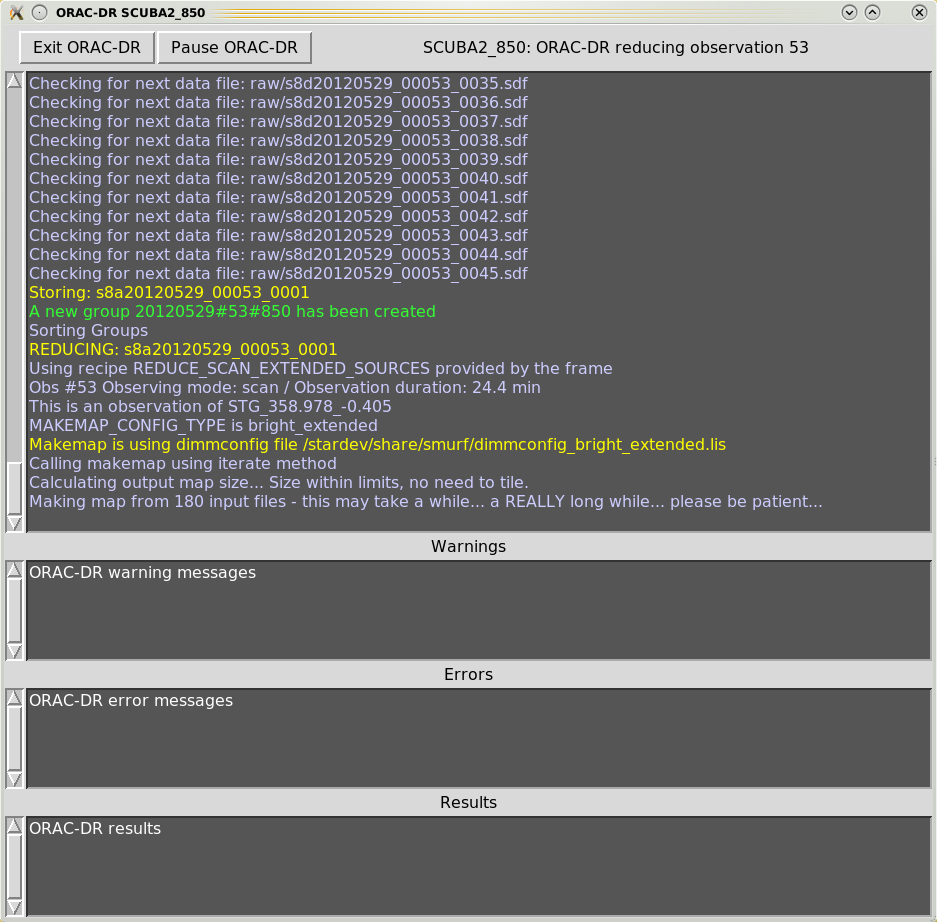
\includegraphics[width=0.7\linewidth]{sc21-pipeline-oracdr-2}
\caption[Output from the pipeline]{The Xwindows output from the \oracdr\
pipeline---here we see the data being reduced with the recipe
REDUCE\_SCAN\_EXTENDED\_SOURCES. The pipeline also reports the name of the
observation being reduced and the duration of the observation. \label{pipeline-oracdr-2}}
\end{center}
\end{figure}

\begin{figure}
\begin{center}
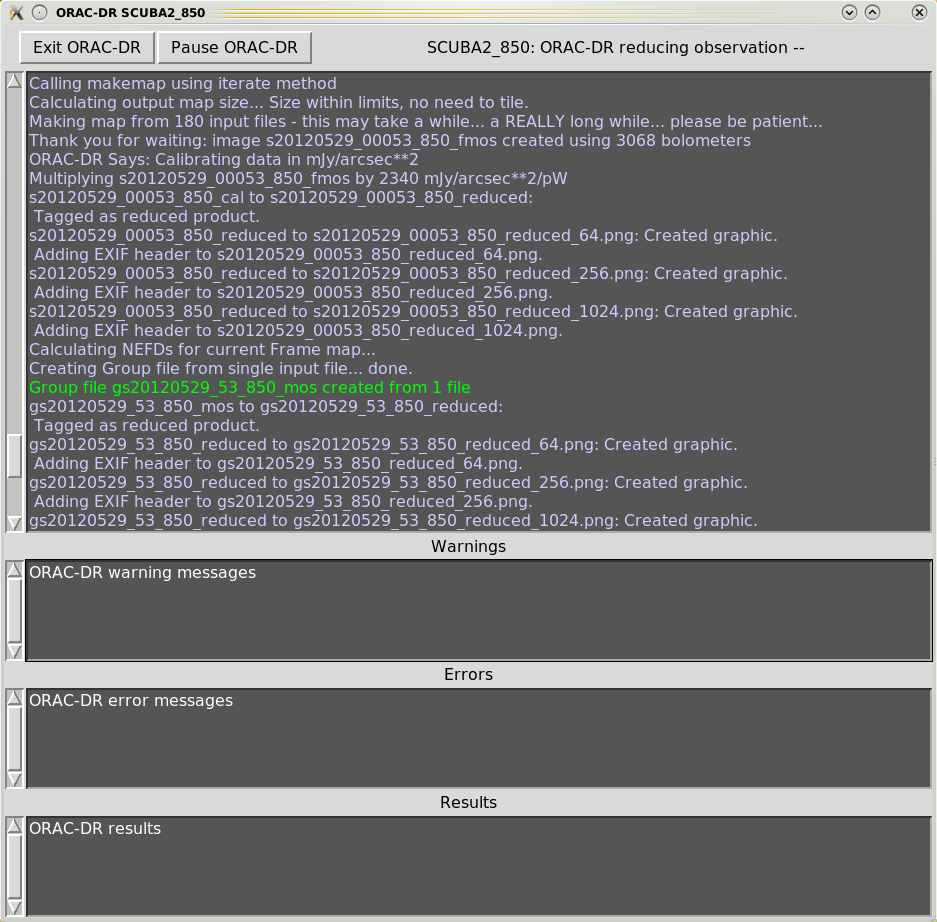
\includegraphics[width=0.7\linewidth]{sc21-pipeline-oracdr-3}
\caption[Output from the pipeline]{The Xwindows output from the \oracdr\
pipeline---here we we see the FCF being applied, the graphics
being created along with a group file (file containing co-added observations
from a single night - if provided). \label{pipeline-oracdr-3}}
\end{center}
\end{figure}


\begin{figure}
\begin{center}
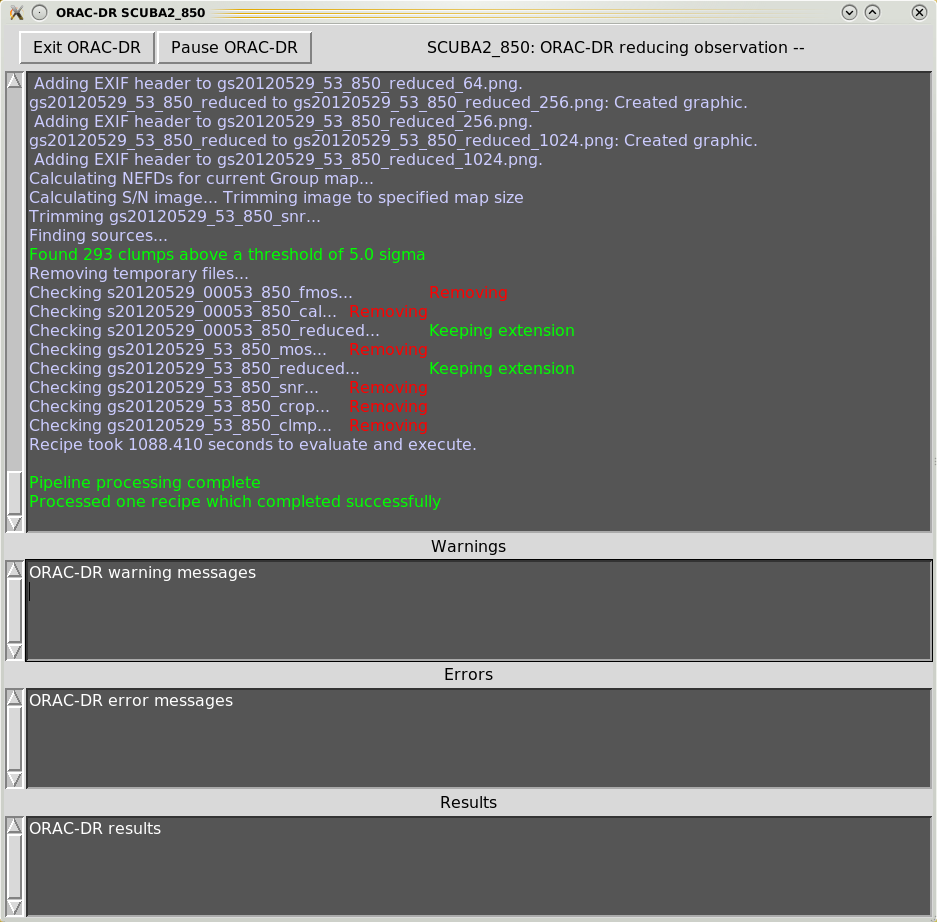
\includegraphics[width=0.7\linewidth]{sc21-pipeline-oracdr-4}
\caption[Output from the pipeline]{The Xwindows output from the \oracdr\
pipeline---here we see the pipeline process has completed. \label{pipeline-oracdr-4}}
\end{center}
\end{figure}




\section{Changing the defaults}
\label{sec:parameterfile}


\subsection{Changing ORAC-DR's behavior}

ORAC-DR's behavior cab be changed on the command line. For help simply type


\begin{terminalv}
% oracdr -help
\end{terminalv}

To run the pipeline and obtain all messages from the Starlink engines
(rather than just ORAC-DR messages) you will need to run with verbose (\emph{recommended})

\begin{terminalv}
% oracdr -loop file -files <list_of_files>  -verbose
\end{terminalv}


To run the pipeline and have the results sent to the screen (\param{s)} and to a
file (\param{f}---the file produced is usually called \file{.oracdr\_NNNN.log}
where NNNN is the current process ID. It is written to \$ORAC\_DATA\_OUT
and is a hidden file) is specified using the \param{-log} command.

\begin{terminalv}
% oracdr -files <list_of_files> -loop file  -log sf -verbose
\end{terminalv}



\subsection{Changing the pipeline recipe}
You can override the recipe set in the header by listing any different
one on the command line when starting \oracdr. For example
\begin{terminalv}
% oracdr -file <list_of_files> -loop file -log sf REDUCE_SCAN_CHECKRMS
\end{terminalv}

You can find out which recipe is set in the data header via the FITS
header \texttt{RECIPE} keyword in any of your raw files.  For
example both of these options will return the same result:
\begin{terminalv}
% fitsval s8a20120725_00045_0003 RECIPE
% fitslist s8a20120725_00045_0003 | grep RECIPE
\end{terminalv}

\subsection{Changing the configuration file}

Although each recipe calls one of the standard configuration files
you can specify your own. You will need to create a recipe parameter
file. This file will set the parameter \param{MAKEMAP\_CONFIG} to be
your new configuration file. The first line must be the name of the
recipe used in the reduction.

For example, to run the pipeline with \drrecipe{REDUCE\_SCAN\_CHECKRMS} with a
configuration file called \file{myconfig.lis}, the recipe parameter file
(\file{mypars.ini}) will look like this.
\vspace{0.2cm}
\begin{terminalv}
[REDUCE_SCAN_CHECKRMS]
MAKEMAP_CONFIG = myconfig.lis
\end{terminalv}

Then run the pipeline calling the parameter file via the
\texttt{-recpars} option.
\begin{terminalv}
% oracdr -file <list_of_files> -loop file -log sf -recpars myparams.ini REDUCE_SCAN_CHECKRMS
\end{terminalv}

\subsection{Parameter file options}

To supply both a new configuration file and a different set of
clump-finding parameters we would update the parameter file
\file{mypars.ini} to look like:

\begin{terminalv}
[REDUCE_SCAN]
MAKEMAP_CONFIG = mynewconfig.lis
FINDCLUMPS_CFG = myfellwalkerparams.lis
\end{terminalv}

Other options we can change in the parameter file include---changing the pixel size

\begin{terminalv}
[REDUCE_SCAN]
MAKEMAP_PIXSIZE = 2
\end{terminalv}

changing output units to mJy/beam

\begin{terminalv}
[REDUCE_SCAN]
CALUNITS = beam
\end{terminalv}

changing output units to mJy/arcsec

\begin{terminalv}
[REDUCE_SCAN]
CALUNITS = arcsec
\end{terminalv}



\section{\xlabel{look_for}What to look out for}
\flushbottom

Once the map-maker has completed you can open your output map using
\gaia\ (see \cref{Figure}{fig:itermap}{this example}). The excerpt in
\cref{Chapter}{sec:manual}{Running the iterative map-maker} shows the
output written to the terminal as you run the map-maker. There are a
number of clues in this output that indicate the status of the
reduction.


\begin{figure}
\begin{center}
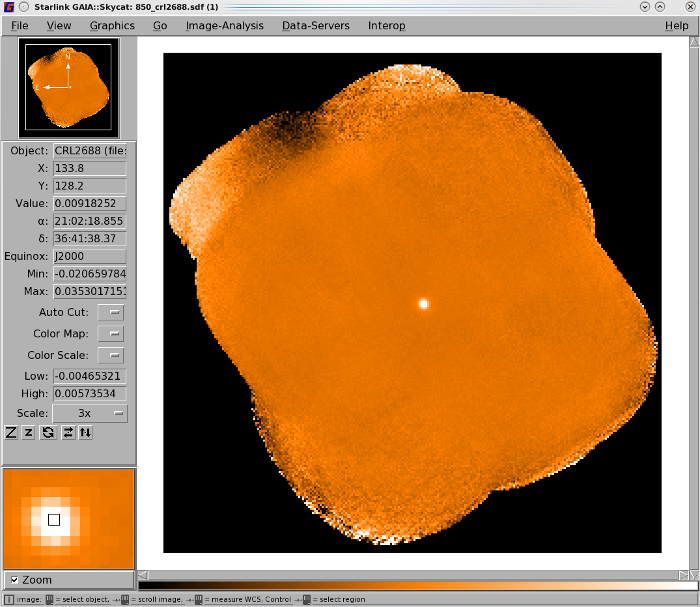
\includegraphics[width=0.7\linewidth]{sc21_crl2688}
\caption[CRL~2688 produced with \makemap]{
  Map of CRL~2688 produced with the \smurf\ task \makemap\ using the
  iterative algorithm with default parameters. \label{fig:itermap}}
\end{center}
\end{figure}

\begin{description}
\item[The number of input files] The first to note is the number of
  input files; it is worth checking this matches your expected
  number. Also summarised are the source name, UT date and scan
  number.

\item[Map dimension] Next the basic dimensions of the data being
  processed are listed near the start of the first iteration. The
  example above has 4\,arcsec pixels---the default at 850$\mu$m.


\item[Chunking] The map-maker then determines if the raw data should
  be split and processed in more than one chunk. In this map the data
  are reduced in one continuous piece: \param{Continuous chunk 1 /
    1}. Chunking is where the map-maker processes sub-sections of the
  time-series data independently and should be avoided if
  possible---see the text box on \latexhtml{Page~\pageref{box:chunk}}{\htmlref{Chunking}{box:chunk}}.
\end{description}


\subsubsection*{Quality statistics}

At the beginning of the reduction, the main purpose of QUALITY
flagging is to indicate how many bolometers are being used. In the
example above you can see that from a total of 5120 bolometers, 1842
were turned off during data acquisition (\texttt{BADDA}). In addition,
136 bolometers exceeded the acceptable noise threshold
(\texttt{NOISE}), while tiny fractions of the data were flagged
because the telescope was moving too slowly (\texttt{STAT}) or the
sample are adjacent to a step that was removed (\texttt{DCJUMP}).

The total number of bad bolometers (\texttt{BADBOL}) is 1984.
Accounting for these, and the small numbers of additionally flagged
samples, 3128.22 effective bolometers are available after initial
cleaning\footnote{The fractional number is due to time-slices being
removed during cleaning. The number of bolometers is then
reconstructed from the number of remaining time-slices.}.


After each subsequent iteration a new `Quality' report is produced,
indicating how the flags have changed. An important flag that appears
in the `Quality' report following the first iteration is \model{COM}:
the DIMM rejects bolometers (or portions of their time series) if they
differ significantly from the common-mode (average) of the remaining
bolometers.

You may note that compared with the initial report, the total number
of samples with good `Quality' (\texttt{Total samples available for
  map}) has dropped from 18634826 to 18273302 (about a 2 per cent
decrease) as additional samples were flagged in each iteration.

Be aware that some large reductions may take many iterations to reach
convergence and you may find significantly fewer bolometers remaining
resulting in higher noise than expected.

\subsubsection*{Convergence}

The convergence criteria \xparam{MAPTOL}{maptol} is updated for each
iteration. The convergence can be checked from the line reporting\\*
\hspace*{0.5cm} \texttt{smf\_iteratemap: *** NORMALIZED MAP CHANGE:
  0.10559 (mean) 2.81081 (max)}

The number to look out for is the mean value. This will have to drop
below your required \param{maptol} for convergence to be achieved.

The default configuration file used in this example executes a maximum
of five iterations, but stops sooner if the change in \param{maptol}
drops below 0.05 (i.e. \param{numiter~=$-$5}). In this example it
stops after five iterations.



\begin{tip}
  You can interrupt the processing at any stage with a single
  \texttt{Ctrl-C}. The map-maker will complete the iteration then
  write out a final science map. Entering \texttt{Ctrl-C} twice will
  kill the process immediately.\widowpenalty=100000
\end{tip}

\section{\xlabel{pl_output}Pipeline output}

The pipeline will produce a group file for each object being
processed. If the pipeline is given data from multiple nights, all
those data will be included in the group co-add using inverse variance
weighting.

The final maps in your output directory will have the suffix
\file{\_reduced}. Maps will be made for individual observations, which
will start with an \file{s} (e.g.
\file{s20140620\_00030\_850\_reduced.sdf}). Group maps, which may
contain co-added observations from a single night, are also produced
which have the prefix \file{gs} and the date/scan of the first input file
(e.g. \file{gs20140620\_30\_850\_reduced.sdf}).

\textbf{Note:} A group file is \emph{always} created, even if only a
single observation is being processed.

Additionally, PNG images are made of the reduced files at a variety of
resolutions.

Another useful feature is that the pipeline will generate a log files
to record various useful quantities. The standard log files from
reducing science data are:

\begin{itemize}
\item \file{log.noise}---noise in the map for each observation and the co-add
(calculated from the median of the error array), and
\item \file{log.nefd}---NEFD calculated for each observation and for
the co-added map(s).
\end{itemize}

\section{\xlabel{cadc}Getting your data from CADC}

The JCMT Science Archive is hosted by The Canadian Astronomy Data
Centre (CADC). Both raw data and data processed by the science
pipeline are made available to PIs and co-Is through the CADC
interface (\url{http://www3.cadc-ccda.hia-iha.nrc-cnrc.gc.ca/jcmt/}).

To access proprietary data you will need to have your CADC username
registered by the EAO and thereby associated with the project code.

An important search option to be aware of is `Group Type', where your
options are Simple, Night, Project and Public. Simple (which becomes
`obs' on the result page) is an individual observation; night means
the group file from the pipeline (these may or may not include more
than one observation; the `Group Members' value will tell you); and
the project option is generated if an entire project has been run
through the pipeline and identical sources across the project are
co-added into master group files.


